%&tex
\documentclass{standalone}

\usepackage[dvipsnames]{xcolor}

\usepackage{tikz}
\usetikzlibrary{positioning,shadows}
\usetikzlibrary{arrows,chains,positioning,scopes,shapes.geometric,shapes.misc,shadows,decorations.markings}
\usepackage{bm}


\begin{document}

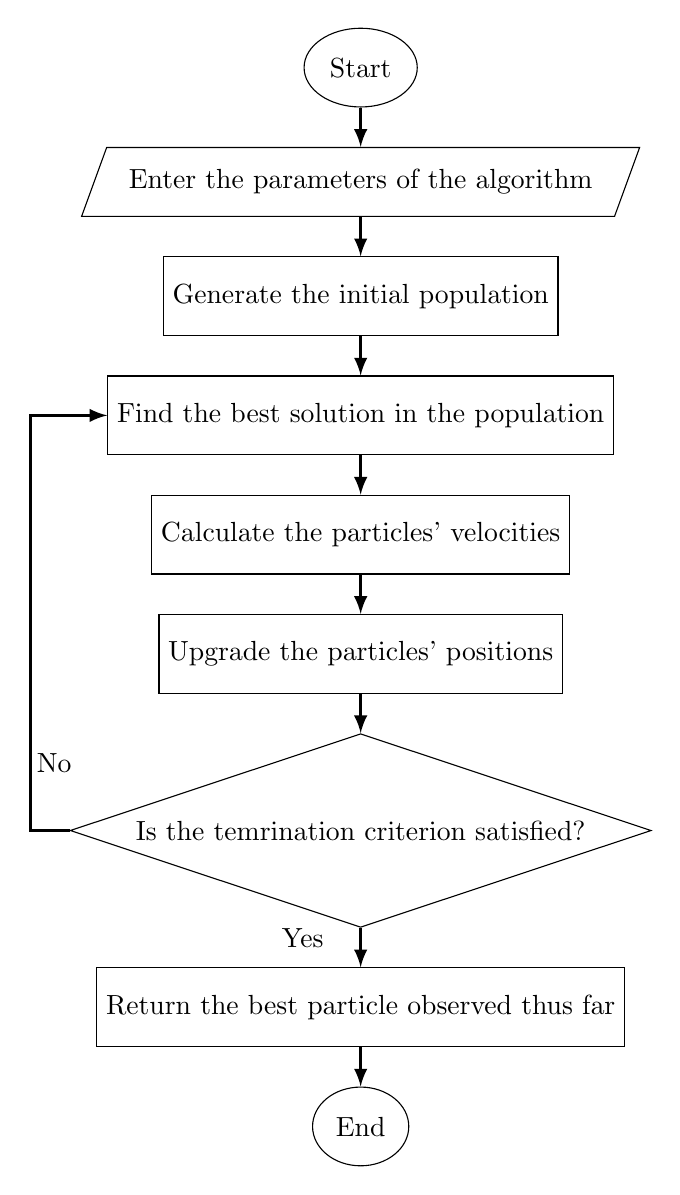
\begin{tikzpicture}

	% \draw[help lines, step=1cm,gray!20] (-10,-5) grid (10,5);

	\node[draw,
	ellipse,
	fill=white,
	minimum width=0.5cm,
	minimum height=1cm] (START) at (0,0) {Start};

	\node[draw,
	trapezium,
	fill=white,
    trapezium left angle=70,
    trapezium right angle=110,
    inner xsep=8pt,
    inner ysep=8pt] (B1) [below = 0.5cm of START] {Enter the parameters of the algorithm};

	\node[draw,
	rectangle,
	fill=white,
	minimum width=0.5cm,
    minimum height=1cm] (B2) [below = 0.5cm of B1] {Generate the initial population};

	\node[draw,
	rectangle,
	fill=white,
	minimum width=0.5cm,
    minimum height=1cm] (B3) [below = 0.5cm of B2] {Find the best solution in the population};

	\node[draw,
	rectangle,
	fill=white,
	minimum width=0.5cm,
    minimum height=1cm] (B4) [below = 0.5cm of B3] {Calculate the particles' velocities};

	\node[draw,
	rectangle,
	fill=white,
	minimum width=0.5cm,
    minimum height=1cm] (B5) [below = 0.5cm of B4] {Upgrade the particles' positions};

	\node[draw,
	diamond,
	fill=white,
	minimum width=0.5cm,
    aspect=3.0,
    minimum height=1cm] (B6) [below = 0.5cm of B5] {Is the temrination criterion satisfied?};

	\node[draw,
	rectangle,
	fill=white,
	minimum width=0.5cm,
    minimum height=1cm] (B7) [below = 0.5cm of B6] {Return the best particle observed thus far};

	\node[draw,
	ellipse,
	fill=white,
	minimum width=0.5cm,
    minimum height=1cm] (END) [below = 0.5cm of B7] {End};

    \draw[-latex, very thick] (START.south) -- (B1.north);
    \draw[-latex, very thick] (B1.south) -- (B2.north);
    \draw[-latex, very thick] (B2.south) -- (B3.north);
    \draw[-latex, very thick] (B3.south) -- (B4.north);
    \draw[-latex, very thick] (B4.south) -- (B5.north);
    \draw[-latex, very thick] (B5.south) -- (B6.north);
    \draw[-latex, very thick] (B6.south) -- (B7.north);
    \draw[-latex, very thick] (B7.south) -- (END.north);
    \draw[-latex, very thick] (B6.west) -- ++(-0.5cm,0cm) |- (B3.west);

    \node[] (t1) [above left = 0cm and 1.7cm of B6] {No};
    \node[] (t2) [below left = 0.5cm and -1.5cm of B6] {Yes};

\end{tikzpicture}

\end{document}
